\documentclass[english,a4paper,11pt]{article}

\usepackage[utf8]{inputenc}
\usepackage{natbib}
\usepackage{graphicx}  %%% for including graphics
\graphicspath{{./images/}}
\usepackage{url}       %%% for including URLs
\usepackage{times}
\usepackage[margin=25mm]{geometry}

%%% custom packages
\usepackage{booktabs}
\usepackage{tabularx}
\usepackage{hyperref}
\usepackage[autostyle=true]{csquotes}
\usepackage{xpatch}
%%% custom packages

\title{Sentiment Analysis of Soldiers' Tweets - Comparison with civilians (TBC)}
\date{\today}

\author{
  Sumit Mukhija, Rachit Rastogi,\\
  Chao Chen, Chen Wang, Chetan Prasad\\
  School of Computer Science and Statistics, Trinity College Dublin\\
  \texttt{\{mukhijas, rrastogi, chenc1, wangc5, cprasad\}@tcd.ie}
}

\begin{document}
\maketitle
\thispagestyle{empty}
\pagestyle{empty}

\begin{abstract}
  The concern to veterans' mental health should be made. Existing works show that
  mental health changes caused by wars can be reflected in linguistic features of
  the social media texts. In order to detect and compare those changes we collected
  data from 20 soldiers' tweets and examined them with a list of positive and negative
  adjectives to identify the polarity and do a comparison with normal users'
  tweets. The total counts of tweets vary from 57 to 39,000. We identified the
  difference between normal users and soldiers and we did a close look to the
  result with discussion. \\
  \textbf{Keywords:}
\end{abstract}

\section{Introduction}

Social media platforms and microblogging websites are some of the most popular
online stages for people to express their views. Twitter, undeniably is one of
the leading applications in this assortment. People use Twitter to post their
real-time opinions in the form of tweets. These tweets can be analyzed and
certain inferences can be extracted. These inferences can subsequently be used
for academic and business purposes.

One of the primary reasons that make Twitter a feasible choice is the diverse
nature of the users. In this research, we intend to analyze and compare the
tweets of the war-veterans and the general public. We believe wars have an
impact on soldiers’ psychological and emotional states. We try to prove this
hypothesis by comparing their tweets to the tweets posted by the civilians.

We collect public data using Twitter API and then process and count the words
with a list of positive and negative adjectives to predict the polarity of the
tweets. Then we examine a randomly collected dataset to compare the difference
between tweets by veterans/soldiers and civilians.

(TBC due to the experiment implementation)

The remainder of the paper is organized as follows. We examine on
the literature related to the topic, with papers related to previous works on
the mental health of veterans, available databases on sentiment analysis and
previous works done on sentiment analysis on social media in Section 2. In Section 3, we
introduce our dataset and the experiment done on the dataset, with the results
we have. In Section 4, we have a deep look into the result and bring the
discussion. In Section 5 and 6, we conclude and bring up future works needed
for the topic.

\section{Background}

\subsection{Previous Work on Mental Health of Veterans}

In order to make a medical diagnosis for patients, psychologists often use the
linguistic content and expression of patients to judge their emotional changes
and mental state according to previous research in psychology and linguistic.
The clinical diagnosis efficiency has been greatly improved because of the
progress of science and technology, especially in computational linguistics.
In addition, the widespread of social media such as Facebook, Twitter and
Instagram, has provided mental researchers with a large scale of data.
Therefore, they could easily use the collected dataset and machine learning
techniques for sentiment analysis. Linguistic contents which users posted on
social media have been proved to be the basis for evaluating a person's mental
state (\cite{becauseIwastoldsomuch} and \cite{GUNTUKU201743}). However,
the majority of research targets are normal people.

In this paper, veterans will be regarded as research targets. Westgate in
\cite{doi:10.1176/appi.ps.201400283} has come up with a method about the evaluation
of veterans' suicide risk. This paper will concentrate on analyzing
the impact of the war on veterans' mental state through the Twitters posted by
themselves before and after the war instead of focusing on the prediction of
the suicide risk of veterans. In addition, the comparison with the twitters
released by ordinary users will be presented. Finally, comprehensive
sentiment analysis of veterans will be summarized.

\subsection{Available Database on Sentiment Analysis}

Sentiment analysis is a very useful method for analysing the sentiment of an
article, tweets or reviews. The advances in Natural Language processing and
linguistic research have led to the development of different methods of
sentiment analysis. The sentiment analysis is an integral part of our work and
it is the fulcrum on which our hypothesis hangs on. Determining not just the
sentiment of a text but even the topic (\cite{10.1145/1645953.1646003}) on which
it is written on is one of the interesting works in this field. Another work
makes use of the lexicons in the text and word dictionaries to extract the
sentiment behind it (\cite{10.5555/2002472.2002491}). There is another work that
trains a model to learn not just the words but to also capture the sentiment
behind it (\cite{taboada2011lexicon}).

In this work, we do sentiment analysis on tweets and we compare the tweets of
two types of users. We utilise a simple model which basically just classifies
the tweets into Happy and sad/depressing sentiments. This is sufficient
considering our work is to identify the difference in the mental states between
the soldiers who have served in wars and common people.

\subsection{Sentiment Analysis on Social Media}

Emotion and sentiment are treated as different concepts in psychology. The
definition of \enquote{emotion} is a complex psychological state, which plays an
important role in operating motivators. For \enquote{sentiment}, it is created based on
emotion to refer to a mental attitude. A survey providing more information can
be referred to by \cite{yue2018survey}.

In sentiment analysis, the typical task is finding the polarities of the given
texts. The tests are probably positive, negative or neutral. The approach is
often counting the word using and produce scores due to the lexicons.

The combination of data mining and machine learning techniques play an important
role in sentiment analysis on social media. There are mainly two approaches -
based on users' social activities and based on linguistic features of
user-generated texts. The sentiment analysis mainly focuses on short texts(tweets)
generated from Twitter accounts, since most of the data is public by default and
easy to obtain online. Also, the tweets are short(limited to 280 characters) and
often appears with spelling mistakes and slangs. A tweet often comes with other
features like spreading tweets(retweet) from other accounts. These mentioned
above makes the analysis on tweets a paradigm to explore.

\cite{robustTwitter2010Luciano} produced an approach to automatically detect
sentiment on tweets with metainformation as retweets, hashtags, replies,
punctuations and emoticons. They also leveraged sources of noisy
labels as their training data to test the robustness.

\cite{agarwal2011sentiment} examined sentiment analysis on Twitter data with POS-
specific prior polarity features, the lexicon features and also the meta
features. They designed a tree representation of tweets and used a partial tree
kernel to calculate the similarity between two trees.

\cite{opinionMiningLiang2013} developed a Unigram Naive Bayes model for
sentiment analysis on Twitter data. The Mutual Information and $\chi^2$ feature
extraction method were used to eliminate unwanted features, and then predictions
were made on the tweets whether they were positive or negative. They found that
the most important features are those combining prior polarity of words with
their POS tags.

\cite{bhavsar2019sentiment} used a dataset from Kaggle and classify the people
emotions based on positive and negative reviews. The model they produced achieved
high accuracy on a large dataset.

The International Workshop on Semantic Evaluation(also known as SemEval)
started holding tasks related to sentiment analysis on social media since 2013.
The rankings of each tasks are made public also with solutions. A list of task
can be found in Table.\ref{table:SemEvalTasks}. % TODO task table

% TODO chage the table, kept as a example on table

\begin{table}[h]
  \caption{The tasks of SemEval on sentiment analysis of tweets}
  \label{table:SemEvalTasks}
  \centering
  \renewcommand{\tabularxcolumn}{m} % we want center vertical alignment
  \begin{tabularx}{\textwidth}{l >{\raggedright}X}
    \toprule
    \textbf{Workshop} & \textbf{Task}
    \tabularnewline \midrule
    SemEval-2013
    &
    Task 2: Sentiment Analysis in Twitter (\cite{SemEval2013Task2})
    \tabularnewline \hline
    SemEval-2014
    &
    Task 9: Sentiment Analysis in Twitter (\cite{SemEval2014Task9})
    \tabularnewline \hline
    SemEval-2015
    &
    Task 10: Sentiment Analysis in Twitter (\cite{SemEval2015Task10})\\
    Task 11: Sentiment Analysis of Figurative Language in Twitter
    (\cite{SemEval2015Task11})
    \tabularnewline \hline
    SemEval-2016
    &
    Task 4: Sentiment Analysis in Twitter (\cite{SemEval2016Task4})\\
    Task 6: Detecting Stance in Tweets (\cite{SemEval2016Task6})
    \tabularnewline \hline
    SemEval-2017
    &
    Task 4: Sentiment Analysis in Twitter (\cite{SemEval2017Task4})\\
    Task 6: \#HashtagWars: Learning a Sense of Humor (\cite{SemEval2017Task6})
    \tabularnewline \hline
    SemEval-2018
    &
    Task 1: Affect in Tweets (\cite{SemEval2018Task1})\\
    Task 3: Irony Detection in English Tweets (\cite{SemEval2018Task3})
    \tabularnewline \hline
    SemEval-2019
    &
    Task 5: HatEval: Multilingual Detection of Hate Speech Against Immigrants
    and Women in Twitter (\cite{SemEval2019Task5})\\
    Task 6: OffensEval: Identifying and Categorizing Offensive Language in
    Social Media(\cite{SemEval2019Task6})
    \tabularnewline \bottomrule
  \end{tabularx}
\end{table}

\section{Experiment and Results}

\subsection{Experiment Setup}

\subsubsection{Data Collection}

% TODO may need to update the last access date in ref.bib
We use TWINT by \cite{twint} as our data collection tool.
All the data can be accessed publically so there are no ethic considerations.

Numerous strategies considered in an attempt to procure data that belonged to
the war veterans. Transcripts of podcasts and YouTube videos involving accounts
of wars from the veterans, books that were written by the ex-servicemen, the
public dataset that had diaries, and letters of first world war soldiers were a
few sources. However, as an inference, all of these sources were highly specific
to the negative aspects and impacts of war and eventually would add bias to the
data.

On account of being a platform that is widely used by a large number of
service-men and the civilians, Twitter was selected as the platform to extract
data. Several verified Twitter pages linked to the US Army were manually analyzed
and a few profiles of the veterans were used as an initial set. Fitting
representation was ensured by selecting 6 veterans belonging to all the genders.
There was also no divide on the number of Tweets. The initial set had Twitter
profiles with as few as 57 tweets and as many as 39,000 tweets. The succeeding
veterans were picked by scouring through the followers of the veterans in the
original set based on some keywords like the army, us-army, military in their
bio.

A collection of 20 veterans was used for the initial proof of concept. However,
we intend to execute the study with 100 soldiers and 100 civilians.

Similarly, 6 civilians were selected with variations in age, sex, and the number
of tweets. The profiles from the initial set were later parsed to get random
followers. A collection of 20 commoners was used for the initial small-scale
proof of concept.

\subsubsection{Data Process and Analysis}

Once the data is gathered and saved in the CSV format, we then start processing
the gathered data where we come up with a set of results to prove our
hypothesis. Sentiment analysis can be broadly categorized into two kinds, based
on the type of output the analysis generates. Under our processing, we are
trying to label text to be under "positive" and "negative". Here we take into
account the tweets of all the selected veterans from our data and then run an
analysis to gather information of there sentiments braking then into two parts,
that is world count of how much words they have used are under the world cloud
of being "Happy", and the same for the one under "Sad". This identical analysis
is then run on tweets by ordinary people. Finally, we will categorise these
words to check the two sets of results which will ultimately help us identify
an individual being in the state of depression with respects to the number of
words count of "positive" and “negative" results.

The initial step was to make a sack of remarkable words. One significant
perception that we went over was that not everyone of a kind word is significant
for our handling. Thus, we focused on descriptive words which are profoundly
educational of positive and negative assessments. The next steps that we took
under processing our data were (1) Removing punctuation (2) Tokenizing (3)
Removing stop words (4) Generating tuple and (5) Finally, extracting the
adjectives.

The first step is to remove punctuation followed by Tokenizing which is the way
toward separating a goliath string into a rundown of words. “NLTK”, a python
library is used for this process. “Stop words”, where pull-out, as they do not
change any meaning of a sentence hence, can be ignored. Tuples were generated
with each word and ts part of speech. Finally, the adjectives were extracted
from the tweets of both the veterans and the civilians. And was then compared
with the word cloud that was created.

Finally, we compared the count of the positive and negative words used by the
two sets of people to come up with a result that displayed whether the veterans
were targeted to depression and suicidal.

The sequence of actions can be refered to Figure \ref{pic:workflow}.

\begin{figure}[h]
  \centering
  \caption{Sequence of actions in the experiment}
  \label{pic:workflow}
  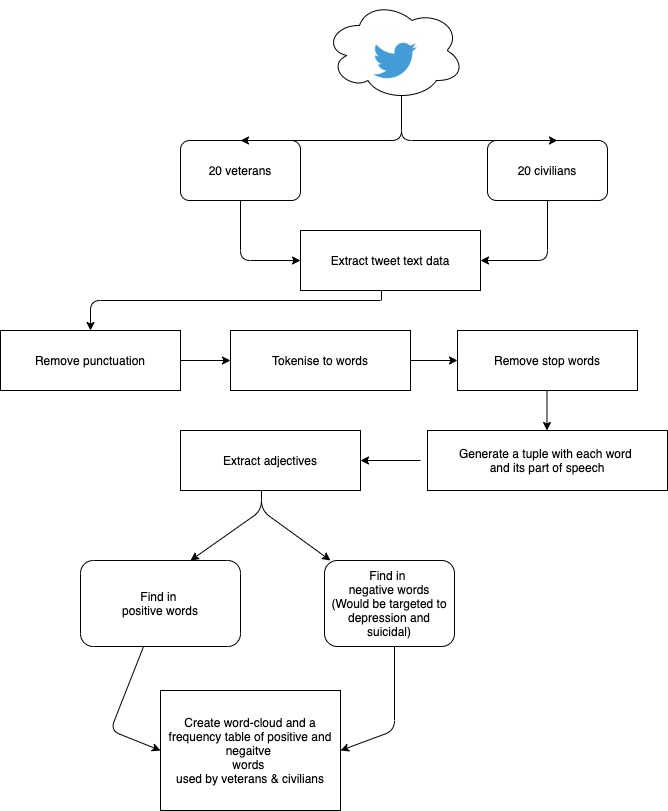
\includegraphics[width=0.75\textwidth]{twitter_workflow}
\end{figure}

\subsection{Results}

\section{Discussion}

\section{Conclusion}

\section{Future Works}


\bibliographystyle{chicago}
\bibliography{ref}

\end{document}
